\usepackage{hyperref}


\chapter{Implementation}\label{ch:implementation}

This chapter presents the created platform; it is structured somewhat similarly to the previous one - firstly, the
audio processing, representation and transfer are discussed, then both the backend and frontend are introduced,
and lastly, the deployment process is shown.
In addition, UML diagrams are provided as an overview of the system.

High level overview can be seen in the following~\ref{fig:system_overview},
~\ref{fig:backend},~\ref{fig:frontend} diagrams.

\begin{figure}[htbp]
    \centering
    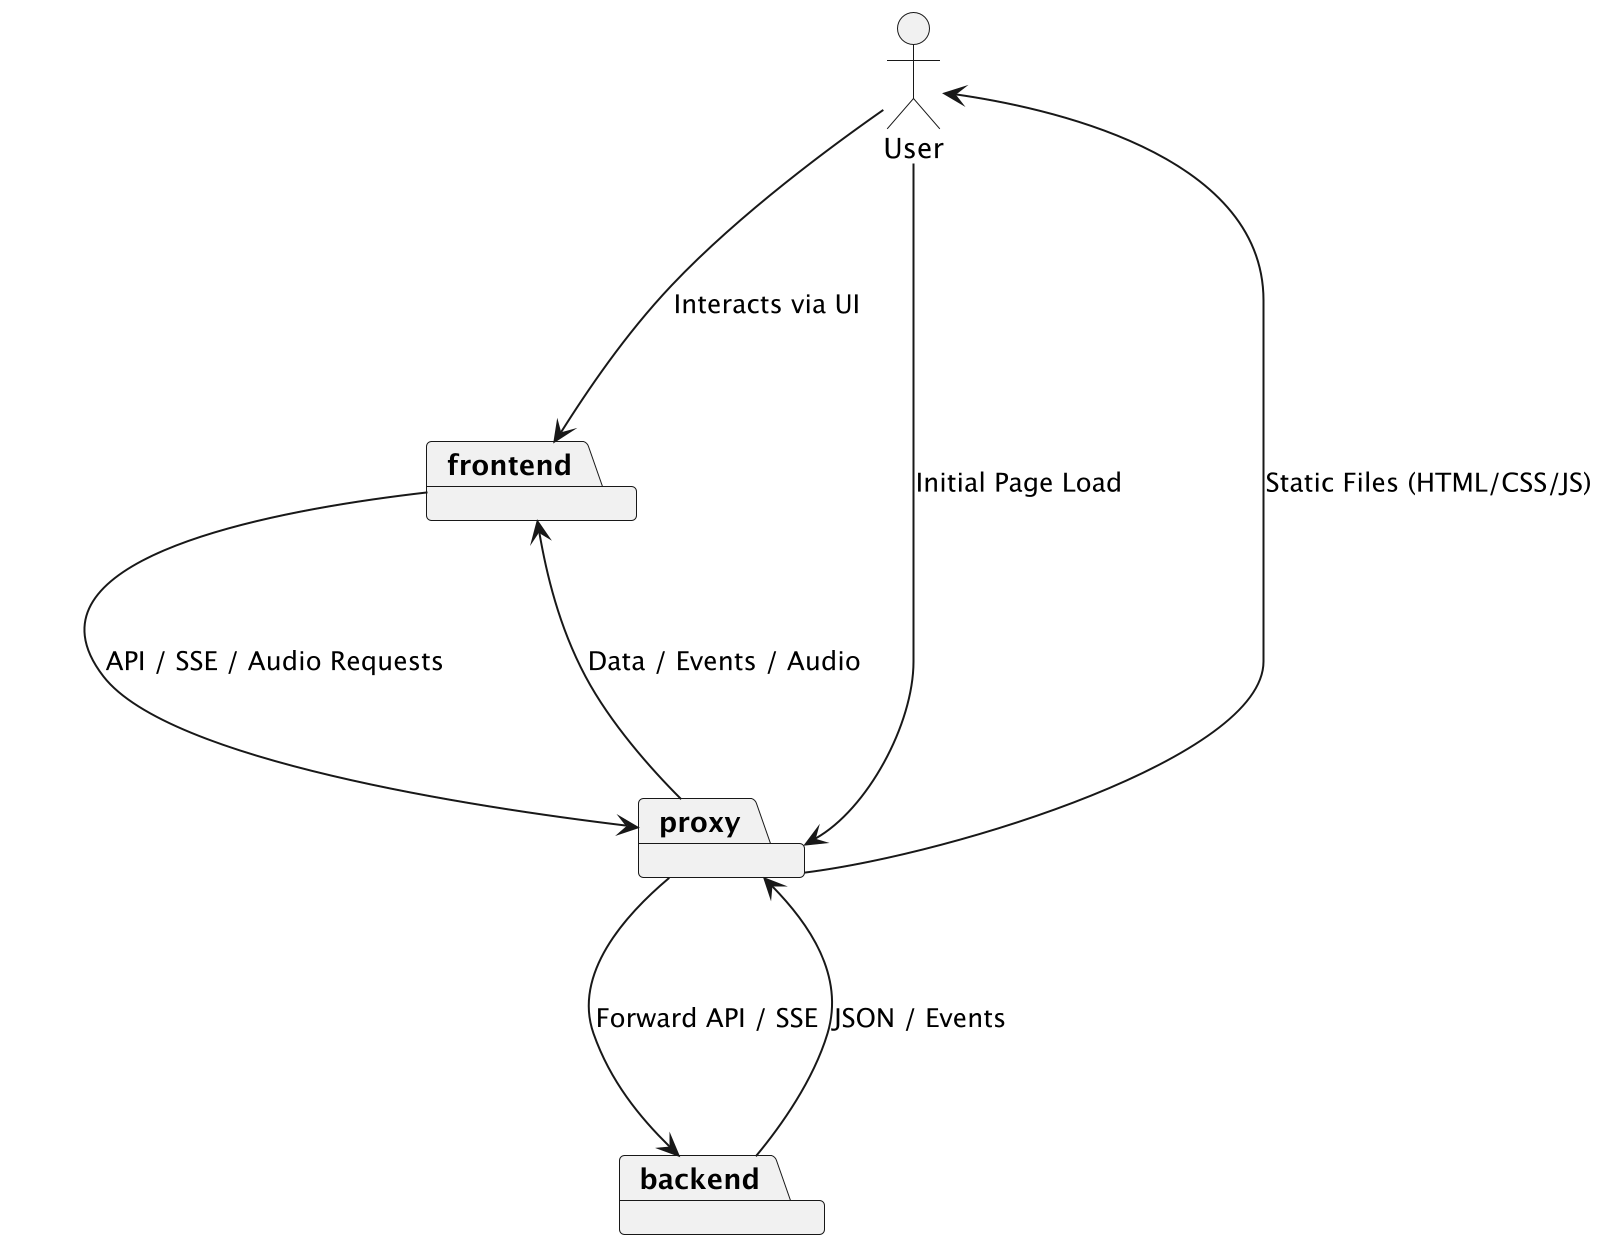
\includegraphics[width=1\textwidth, keepaspectratio]{diagrams/system.png}
    \caption{System Overview}
    \label{fig:system_overview}
\end{figure}

\begin{figure}[htbp]
    \centering
    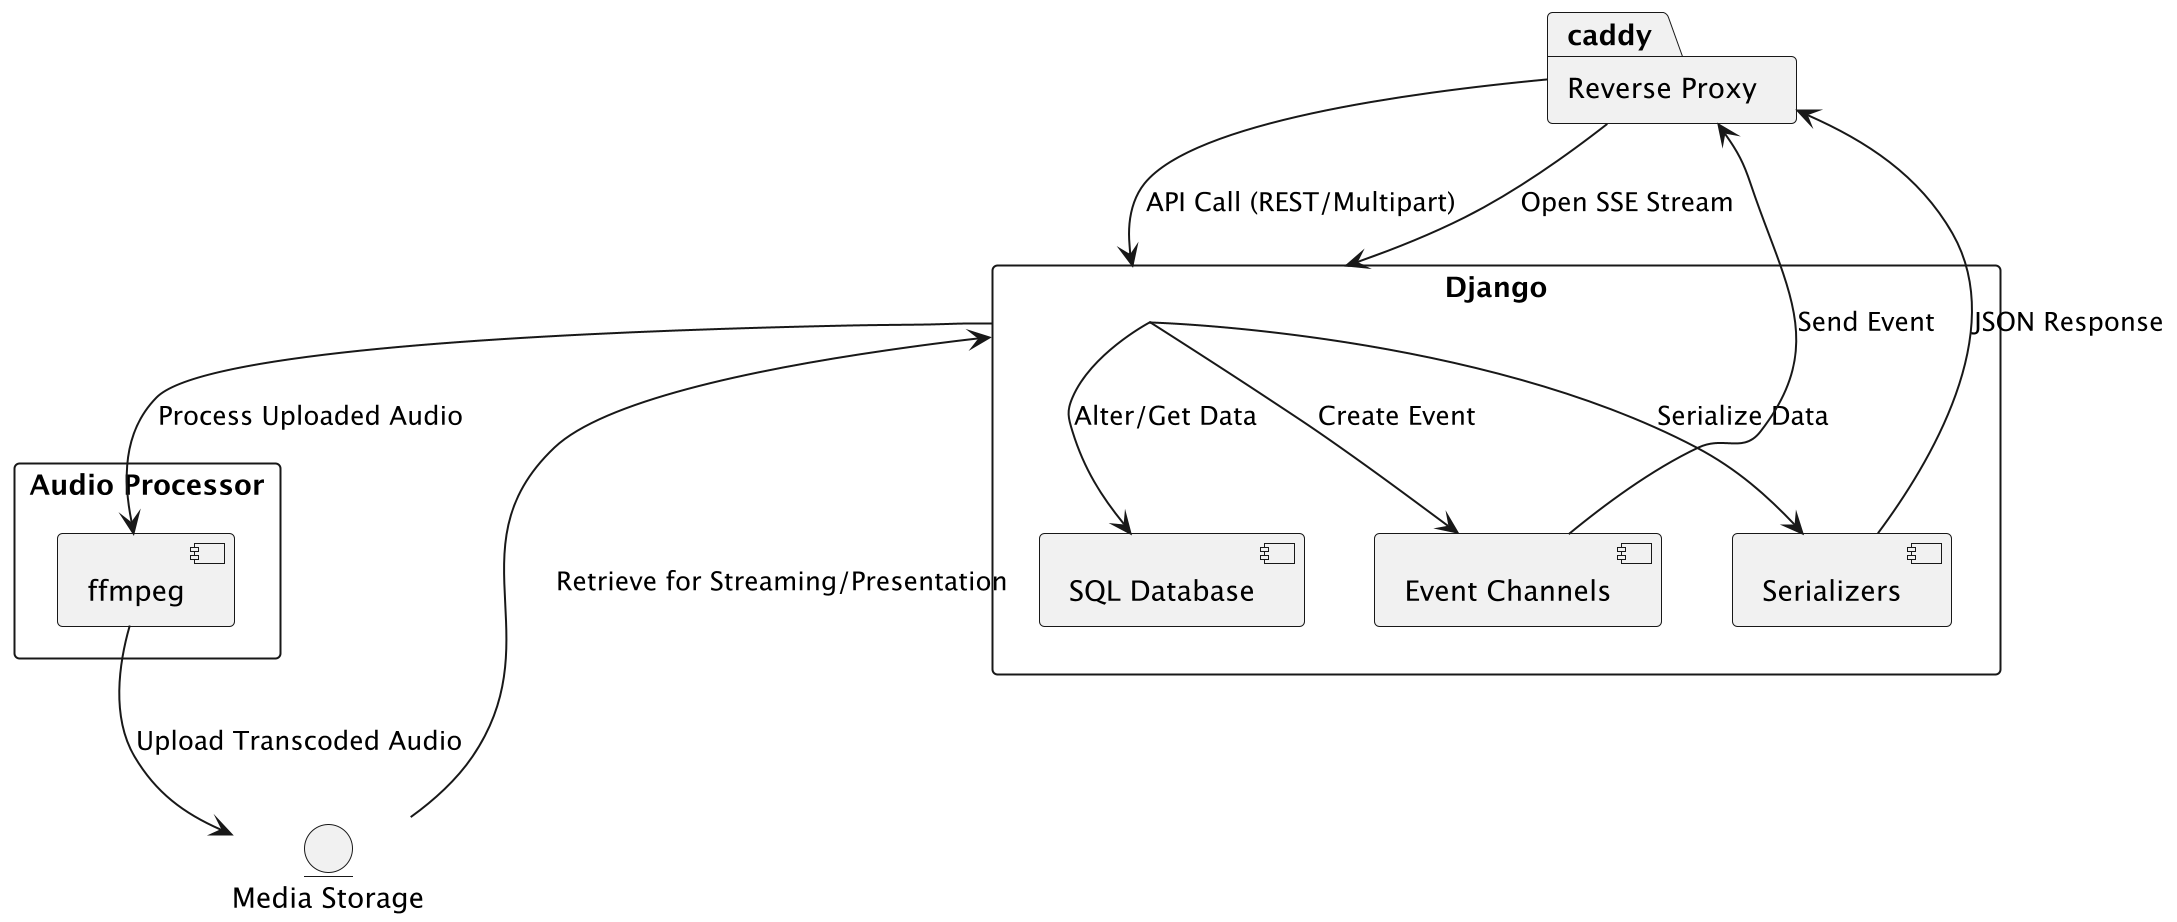
\includegraphics[width=1\textwidth, keepaspectratio]{diagrams/backend.png}
    \caption{Backend}
    \label{fig:backend}
\end{figure}

\begin{figure}[htbp]
    \centering
    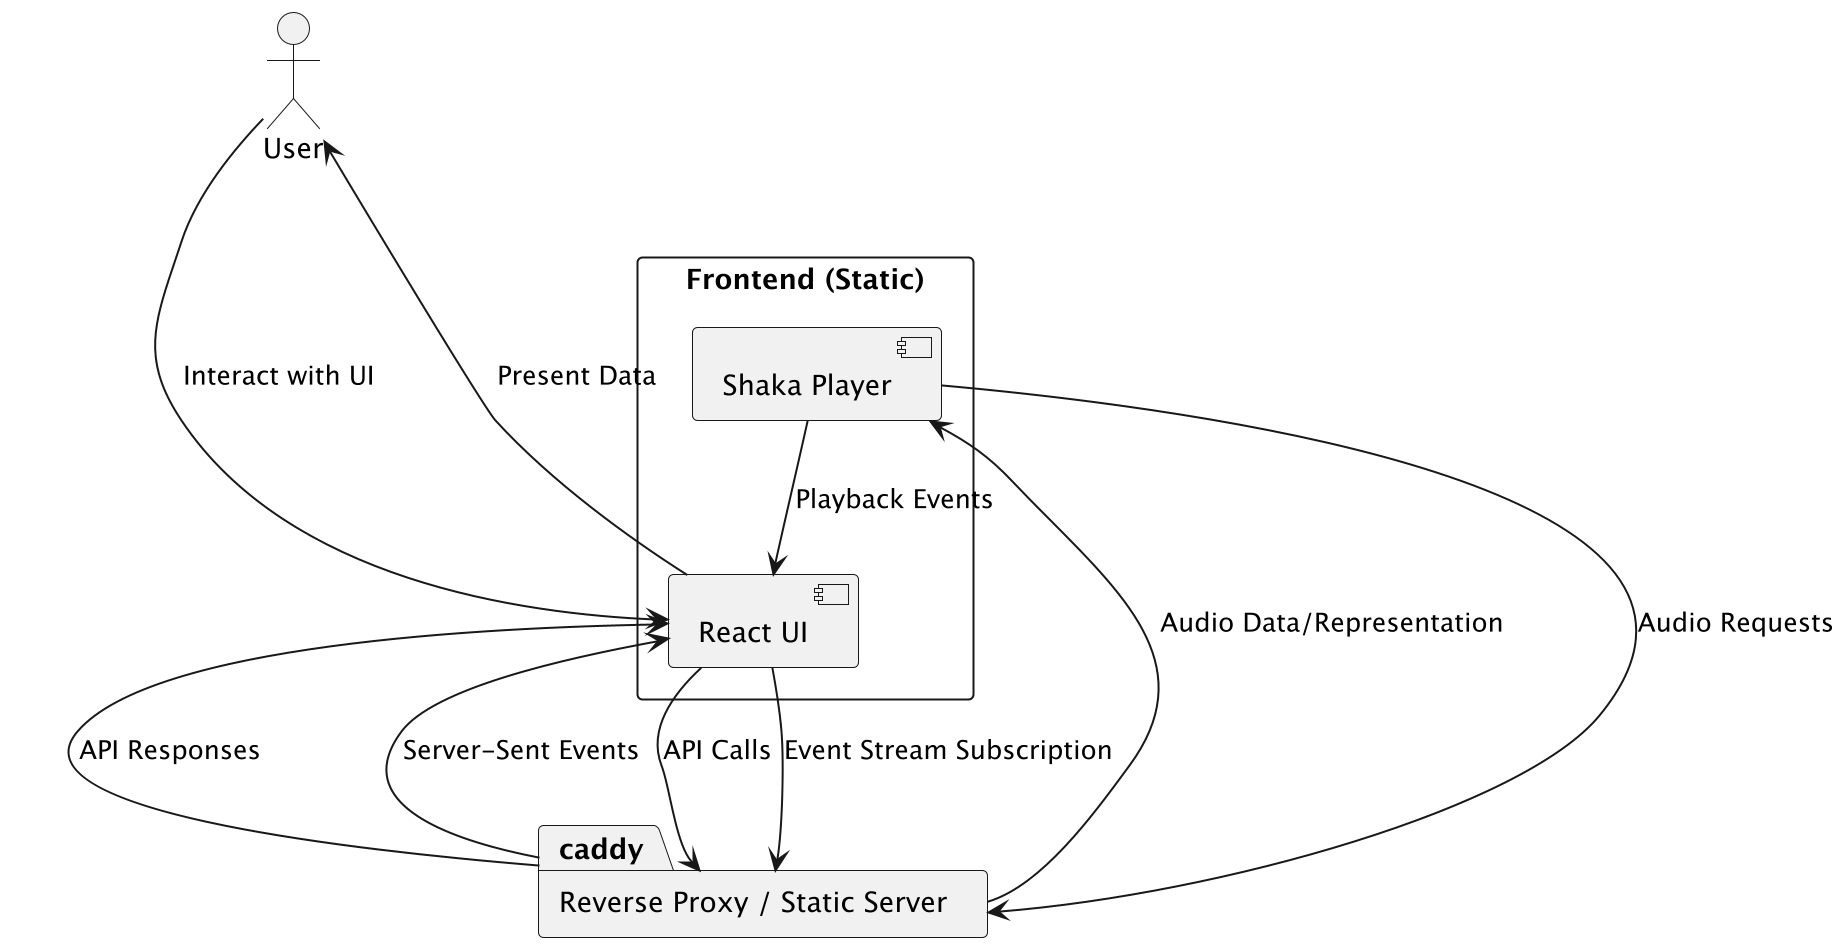
\includegraphics[width=1\textwidth, keepaspectratio]{diagrams/frontend.png}
    \caption{Frontend}
    \label{fig:frontend}
\end{figure}


\section{Audio Processing, Representation and Transfer}

\subsection{Streaming Protocols}
Two protocols were chosen for audio streaming - DASH\cite{dash} and HLS\cite{hls}.
Broadly speaking, they work by breaking the initial audio file into smaller chunks and present them via a manifest,
which is a listing with all available chunks separated by their timecodes. Then it is possible to use that manifest
to request individual chunks instead of fetching the whole file or its byte ranges. Moreover, it is possible to use
different coders and bitrates for the initial file, which would all be arranged together in the resulting manifest, giving
the possibility to choose which chunk will be served next - e.g. in the case of web audio players the next chunk can
be chosen based on multiple parameters, for example, network conditions.

At first, only DASH was considered, as it is codec and container agnostic,
is more efficient for lower bitrates, can stream lossless audio(HLS can only on Apple devices),
has multiple DRM implementations to choose from and many further advantages.
However, Safari does not support it well, and on iOS below 17.1 it does not work due to
Media Source Extensions~\cite{mse,msecaniuse} not being present.
Since Safari is the second most used browser~\cite{browserusage}, HLS is used as well.

After choosing the streaming protocols, it is needed to find the way of converting audio to formats that
they support. Audio representation is discussed first, with tools for the actual audio processing next.

\subsection{Representation}
Usually when audio is recorded, it is initially saved in lossless formats, which are big in size, due to
the absence of any compression. For instance, a the resulting WAV file for a 3-minute stereo audio
recorded with bit depth of 24 bits and a sample rate of 41khz is approximately 42 megabytes, which makes
it very impractical for over-the-net streaming.

Codecs are special programs which aim to reduce the size
while compromising audio quality as little as possible. Most often they take in multiple input parameters
which affect the resulting converted audio, among them is bitrate; the initial bitrate for the raw recorded audio
can be calculated as `Sample rate x Bit depth x Number of channels`.
However, codecs typically use bitrate as a primary input parameter instead of those individual components.
This is because bitrate directly controls the trade-off between audio quality and file size,
making it easier to manage both encoding and playback requirements.
It also abstracts away the internal implementation details, especially in lossy codecs like MP3, AAC, or Opus,
which use perceptual models and compression techniques that aren’t strictly tied to sample rate or bit depth.

The following configuration, based on the official documentation of the respective codec implementations, was selected:
\begin{itemize}[leftmargin=1.5cm]
    \item \textbf{Opus}: 96, 160, and 256 kbps for DASH
    \item \textbf{AAC}: 96, 160, and 320 kbps for HLS
    \item \textbf{AAC-HEv2}: 24 kbps for both HLS and DASH
\end{itemize}
According to performance measurements provided by the codec developers,
these bitrate values offer an optimal balance between audio quality and file size.
Multiple bitrates are included to support adaptive streaming,
allowing web players to dynamically select the most appropriate stream based on current conditions.

\subsection{Processing}
Audio processing is done via \texttt{ffmpeg}\cite{ffmpeg} which is a tool that support both the encoding of audio and the
manifest generation for both streaming protocols. It is written in C and supports multithreading ensuring high speed of
audio conversion.

FFMPEG provides multiple codec implementations, out of which \texttt{libfdk\_aac} and \texttt{libopus} were used.
Again, the choices made were backed by the documentation details~\cite{libfdkaac,libopus}.

In order to integrate it into the backend architecture a small wrapper was written, which can be found in the
\texttt{audio\_processing/ffmpeg\_wrapper.py} and \texttt{audio\_processing/converters.py} files; a class diagram is also
provided~\ref{fig:ffmpeg}.

\begin{figure}[htbp]
    \centering
    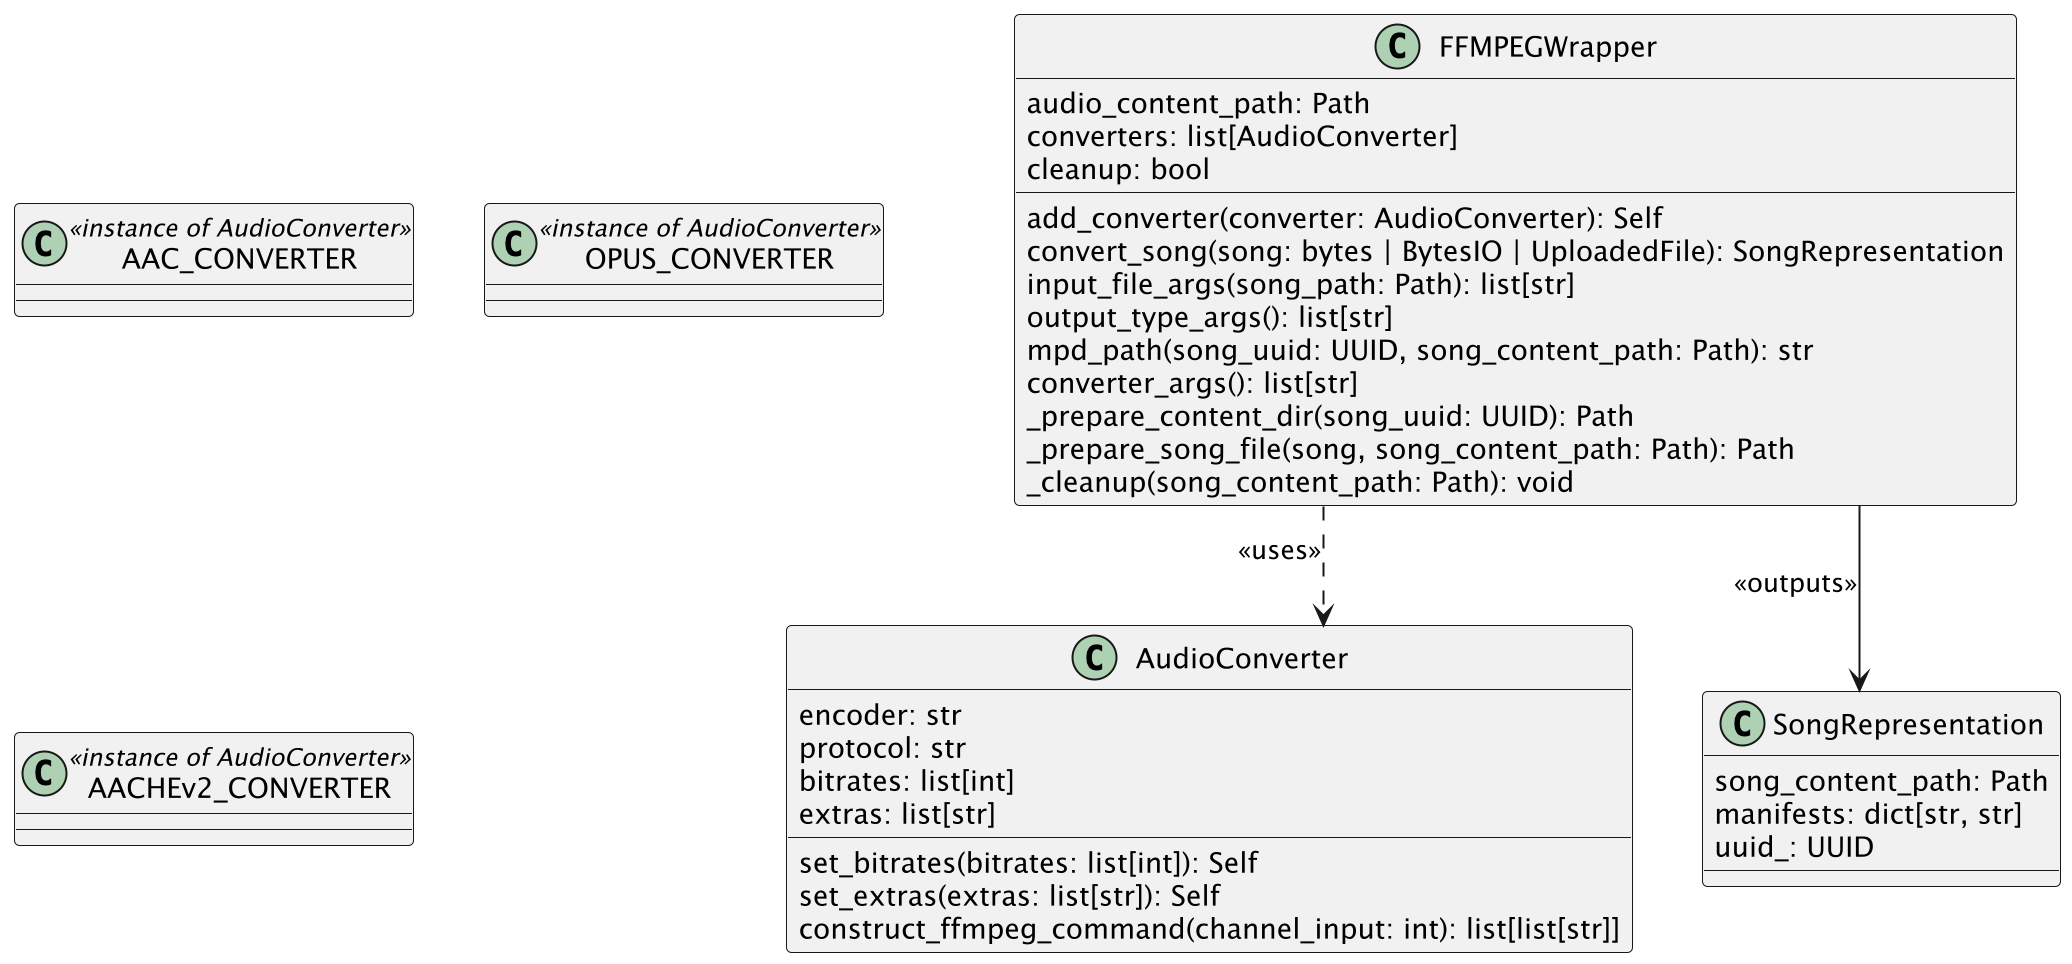
\includegraphics[width=1\textwidth, keepaspectratio]{diagrams/ffmpeg.png}
    \caption{FFMPEG Wrapper}
    \label{fig:ffmpeg}
\end{figure}

There are a couple of packages which already implement a wrapper around the library, however,
they are not used because the needed functionality is minimal and introducing a big
dependency is not necessary. In addition, the more popular and mature package \texttt{ffmpeg-python}\cite{ffmpegpython}
is not maintained anymore and e.g. OpenAI has dropped it as their dependency due to that reason\cite{ffmpegopenai}.

The resulting command for \texttt{ffmpeg} constructed by the wrapper(DASH only, for brevity) looks like this:

\begin{minted}{bash}
ffmpeg -i *input file path*
    -map 0:a -c:a:0 libfdk_aac -profile aac_he_v2 -b:a 24k
    -map 0:a -c:a:1 libopus -b:a 96k
    -map 0:a -c:a:2 libopus -b:a 160k
    -map 0:a -c:a:3 libopus -b:a 256k
    -f dash *output file path for manifest*
\end{minted}

\texttt{-map 0:a} tells \texttt{ffmpeg} to select the audio track(s) from the first input.

\texttt{-c:a:*} specifies the codec for each output audio stream.
The index (e.g., \texttt{:0}, \texttt{:1}, etc.) determines the order of the audio representations
in the output DASH manifest.

As the result, the individual manifests and corresponding chunks are created.
Later on they will be placed under a subdirectory
of Django's media directory, so they can later be served to the frontend audio player.

Having determined, how the audio is going to be processed and represented, backend implementation is
discussed in the further section.


\section{Backend}
The description is organized by individual Django \textit{apps}.
Each app section follows this structure:

\begin{enumerate}
    \item \textbf{Models} – Define the data schema using Django's ORM.
    \item \textbf{Serializers} – Convert Django models or native Python types into
    formats suitable for HTTP transmission (and vice versa).
    \item \textbf{API Endpoints} – Implemented as \textit{views}, these handle HTTP requests,
    apply the relevant business logic, and return appropriate responses.
\end{enumerate}

As a means to simplify the understanding of the underlying architecture, a full class diagram can be
seen first - it encompassed all attributes, methods and relationships of classes~\ref{fig:beclassdiagram}.

\begin{figure}[htbp]
    \centering
    \begin{adjustbox}{angle=90, width=1.4\textwidth, center}
        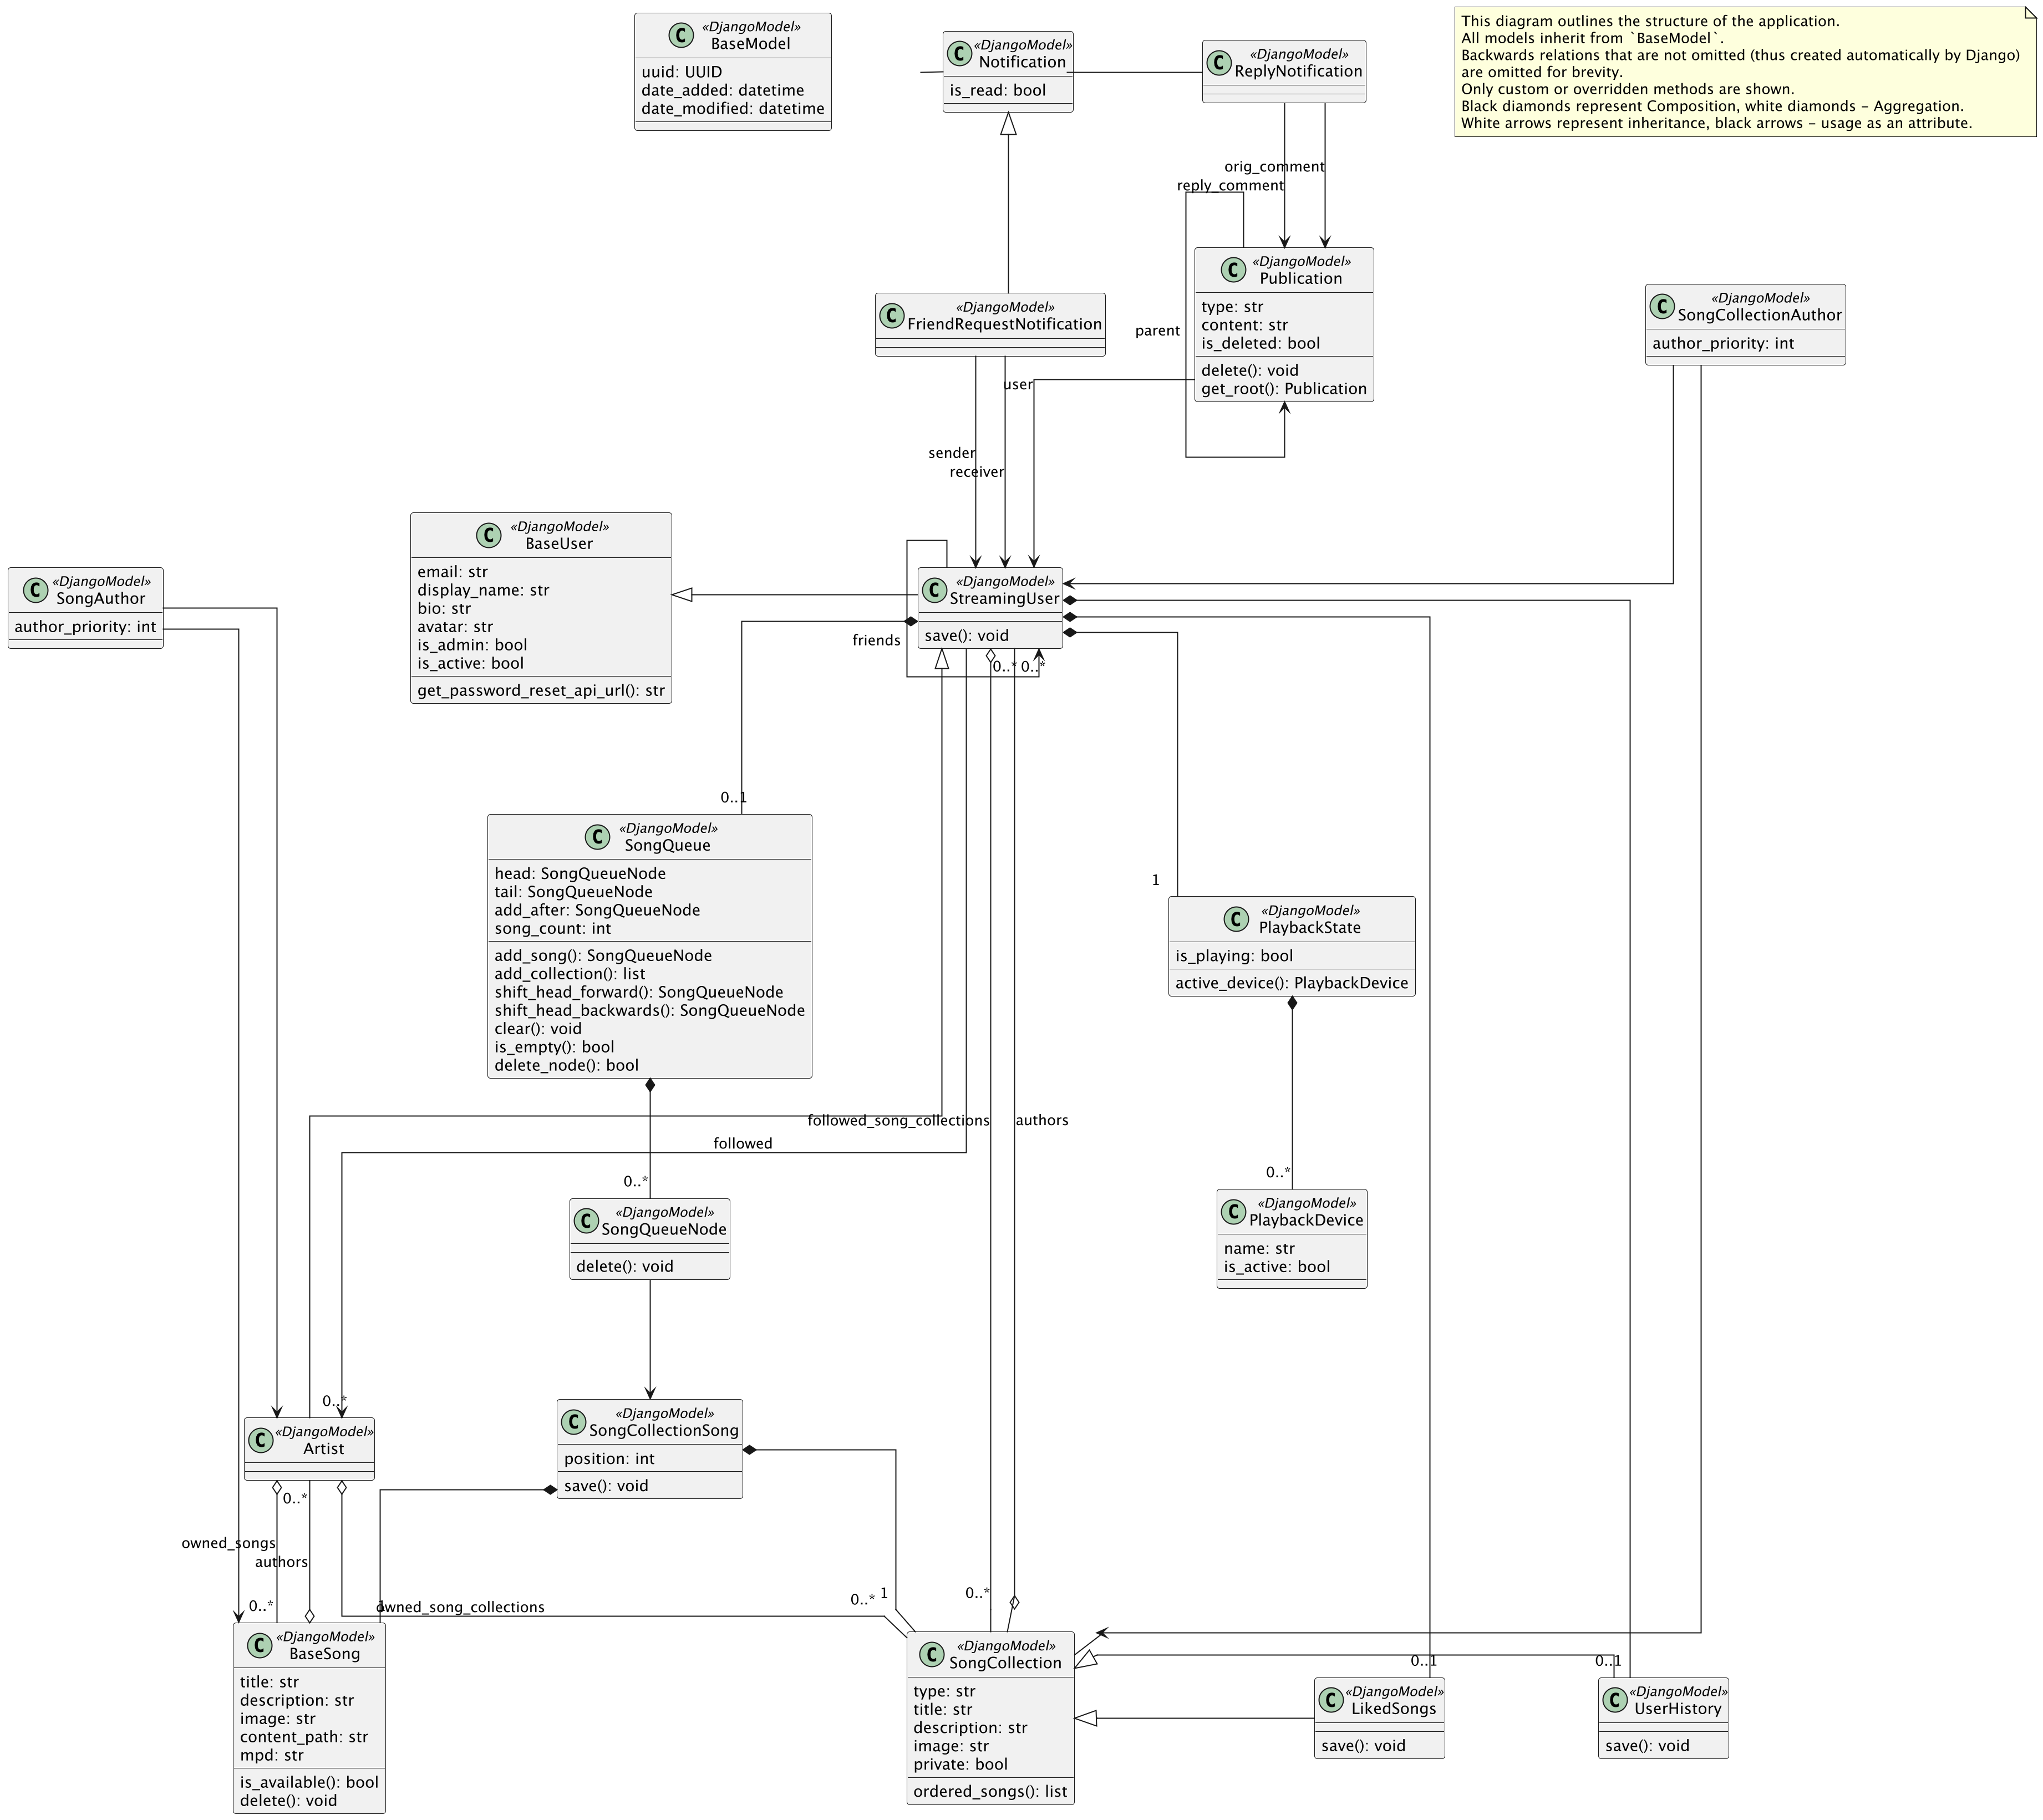
\includegraphics{diagrams/class.png}
    \end{adjustbox}
    \caption{Backend Class Diagram}
    \label{fig:beclassdiagram}
\end{figure}

\subsection{\textit{base}}
In this app the abstract \texttt{BaseModel} class is defined, all other models inherit from it.
It has three attributes - \texttt{uuid, date\_added, date\_modified}. While the latter two are self-explanatory,
\texttt{uuid} deserves an explanation. Since all of the data fetching in frontend will be happening via the REST API,
a unique resource identifier is needed.\\
The drawback of using an \texttt{ID} of the model record, which is added by default for all models by Django,
is the possibility of enumeration attacks~\ref{enumattack} and unauthorized scraping of the web page, since it is
much easier to get an existing ID and simply send requests to API endpoints with an incremented ID value.\\
A serializer for the model is defined here as well, it is also the base class for the serializers of other models.

\subsection{\textit{users}}
User classes and token logic are defined in this app.\\
There are three main User classes:
\begin{itemize}
    \item \texttt{BaseUser} - declares common fields for all other models, such as \texttt{email, display\_name} and others.
    \item \texttt{StreamingUser} - the main class representing an account with privileges to use the streaming platform.\\
    Additional attributes are declared for it, namely:
    \begin{itemize}
        \item Relations to other users: \texttt{friends}, which are other \texttt{StreamingUsers},\\
        friend requests of whom the user has accepted (or the other way around);\\
        \texttt{followed} - the \texttt{Artist}s to the updates of which the User has subscribed.
        \item User-specific Song Collections: \texttt{history} containing all listened Songs,\\
        \texttt{liked\_songs} containing favourited Songs,\\
        and \texttt{followed\_song\_collections} - the Collections which user has saved to their profile.
        \item \texttt{song\_queue} - a special structure containing already listened/to be listened to Songs of the User,\\
        it will be described later in the dedicated app.
    \end{itemize}
    \item \texttt{Artist}: a subclass of \texttt{StreamingUser} with additional capabilities, such as Song uploads.
\end{itemize}

JWTTokens are also customized in this app. The authentication process of individual HTTP requests is made by adding the
token to each request, then parsing and validating it. After validation the supplied User identifier is extracted and
is used to find the existing User record to which the request belongs. Thus, the \texttt{uuid} of the User is added to the token payload, and
the authorization logic, and it is customized to use UUID instead of ID for the user lookup.
The usage of UUID in the token payload will be described in more detail in the frontend section.

Basic serializers for all User models are declared,
allowing for the retrieval of information about specific Users or their creation and updates.

The following views are added as well:
\begin{itemize}
    \item \texttt{UserRetrieveUpdateView}
    \item \texttt{UserCreateView}
    \item \texttt{UserFriendsView}
    \item \texttt{UserFollowedView}
    \item \texttt{UserFriendsCreateDeleteView}
    \item \texttt{ArtistFollowersView}
    \item \texttt{UserEventViewSet}
\end{itemize}

The purpose of all views, except for the last one, could be deduced from their name.\\
UserEventViewSet is a special view used to implement the SSE connection, the details are provided in the next subsection.

\subsection{\textit{sse}}
As was mentioned in \nameref{ch:planning}, \texttt{django-eventstream} package is used for the Server Sent Events
configuration. Internally it works by creating special objects called \textit{channels} to which clients can subscribe
via an HTTP request. Then, when a new event for a specific channel is created,
e.g. via the \texttt{django-eventstream.send\_event()} method, all clients subscribed to that channel
will receive an HTTP response with the specified content.

`UserEventViewSet` listens for incoming SSE connection requests from Users and creates a personalized channel using User's UUID.

Events are mostly used throughout the system to signify to the frontend that some data is stale.
An example of this is the aforementioned `UserFriendsView`, the post request handler of which is defined like this:

\begin{minipage}{\textwidth}
    \begin{minted}{python}
    class UserFriendsCreateDeleteView(APIView):
    ...
    def post(self, request, *args, **kwargs):
        ...
        user.friends.add(sender)
        send_invalidate_event(
            EventChannels.user_events(user.uuid),
            ["user", "friends", str(user.uuid)]
        )
        ...
    \end{minted}
\end{minipage}
\\
\\
Here, the custom \texttt{invalidate\_event} signifies to the frontend that the \texttt{friends} list has changed and should
be refetched.

The \textit{invalidate} logic is used for models that are represented in the frontend,
specifically in view handlers which change data. That way the client always has fresh information.

Event re-delivery is also handled by the package, specifically with this parameter in Django settings:

\begin{flushleft}
    \begin{minted}{python}
    EVENTSTREAM_STORAGE_CLASS = \
        'django_eventstream.storage.DjangoModelStorage'
    \end{minted}
\end{flushleft}

This tells the package to store the events in the database, and in case of network failure or client disconnect they
are redelivered.

Since the SSE part has been explained, it is safe to move on to the main part of the application - the \textit{streaming} package.

\subsection{\textit{streaming}}


%
%\subsection{social}
%
%\subsection{recommendations}
%generic relations content type
%
%\subsection{notifications}
%
%\subsection{audio processing}
%
%\subsection{API}
%versioning, rest practices(and problems, e.g. action endpoints)
%using uuids
%
%
%\section{Frontend}
%
%\subsection{Libs used}
%tanstack query, shadcn, react router, form
%
%\subsection{Components}
%
%\subsection{Interacting with api}
%problems with on leave event
%
%\subsection{sse}
%
%\subsection{player}
%
%
%\section{Deployment}